\section{Review of direct adaptive control}
\begin{frame}
    \frametitle{Outline}
    \tableofcontents[currentsection]
\end{frame}

\begin{frame}
    \frametitle{Deterministic SISO ARMA model}

    SISO ARMA plant model:
    \begin{equation*}
        A(q^{-1}) y(k) = q^{-\drm} B(q^{-1}) u(k)
    \end{equation*}
    where $y(k)$ and $u(k)$ are scalar

    \begin{itemize}
        \item
        $u(k)$ is the control input

        \item
        $y(k)$ is the output

        \item
        $\drm$ is the pure time delay

        \item
        no disturbance
    \end{itemize}
\end{frame}

\begin{frame}
    \frametitle{Model assumptions}

    SISO ARMA plant model:
    \begin{equation*}
        A(q^{-1}) y(k) = q^{-\drm} B(q^{-1}) u(k)
    \end{equation*}
    where $y(k)$ and $u(k)$ are scalar

    \begin{itemize}
        \item
        The polynomials
        \begin{align*}
            A(q^{-1}) & = {\color{red} 1} + a_1 q^{-1} + \cdots + a_n q^{-n} \\
            B(q^{-1}) & = b_0 + b_1 q^{-1} + \cdots + b_m q^{-m}
        \end{align*}
        are co-prime

        \item
        $B(q^{-1})$ is anti-Schur

        \item
        $m$, $n$, and $\drm$ are known

        \item
        $0 < b_{mino} \leq b_0$, where $b_{mino}$ is known
    \end{itemize}
\end{frame}

\begin{frame}
    \frametitle{Control Objectives}
    \begin{enumerate}
        \item[1.]
        \textbf{Pole Placement: } The poles of the closed-loop system must be placed at specific locations in the complex plane

        $ \ $
        \pause

        Closed-loop polynomial:
        \begin{align*}
            A_c(q^{-1}) = B(q^{-1}) A_c^{'}(q^{-1})
        \end{align*}
        where $A_c^{'}(q^{-1})$ is an anti-Schur polynomial chosen by the designer:
        \begin{align*}
            A_c^{'}(q^{-1}) & = {\color{red} 1} + a_{c1}^{'} q^{-1} + \cdots + a_{c(n_c')}^{'} q^{-(n_c')}
        \end{align*}
    \end{enumerate}

\end{frame}

\begin{frame}
    \frametitle{Control Objectives}
    \begin{enumerate}
        \item[2.]
        \textbf{Tracking: } The output sequence $y(k)$ must follow an arbitrary bounded reference sequence $y_d(k)$, which is known

        $ \ $
        \pause

        $y_d(k)$ is generated by the reference model
        \begin{align*}
            {\color{red} A_c^{'}(q^{-1})} y_d(k) = {\color{red}q^{-\drm}} B_m(q^{-1}) u_d(k)
        \end{align*}
        where
        \begin{itemize}
            \item
            $u_d(k)$ is a known \underline{bounded} reference input control input sequence

            \item
            $B_m(q^{-1})$ is chosen by the designer
        \end{itemize}

        $ \ $
        \pause

        Note that $A_c^{'}(q^{-1})$ comes from the pole placement and the reference model delay is the same as the plant delay
    \end{enumerate}
\end{frame}

\begin{frame}
    \frametitle{Reformulated plant dynamics}

    Using the solution of the Diophantine equation
    \begin{equation*}
        A_c^{'}(q^{-1}) = A(q^{-1}) R^{'}(q^{-1}) + q^{-\drm} S(q^{-1})
    \end{equation*}
    we rewrite the plant dynamics as
    \begin{align*}
        A_c^{'}(q^{-1}) y(k) = q^{-\drm} \Big[ R(q^{-1}) u(k) + S(q^{-1}) y(k) \Big]
    \end{align*}
    \pause

    where $R(q^{-1}) = R^{'}(q^{-1}) B(q^{-1})$ and
    \begin{align*}
        R(q^{-1}) & = r_0 + r_1 q^{-1} + \cdots + r_{n_r} q^{-n_r} \\
        S(q^{-1}) & = s_0 + s_1 q^{-1} + \cdots + s_{n_s} q^{-n_s}
    \end{align*}
    \begin{align*}
        n_r & = m + \drm - 1
            & n_s & = \max \{ n-1, n_c' - \drm \}
    \end{align*}

\end{frame}

\begin{frame}
    \frametitle{Reformulated plant dynamics}

    So far, we know that
    \begin{align*}
        A_c^{'}(q^{-1}) y(k) & = q^{-\drm} \Big[ R(q^{-1}) u(k) + S(q^{-1}) y(k) \Big] \\
        R(q^{-1}) & = r_0 + r_1 q^{-1} + \cdots + r_{n_r} q^{-n_r} \\
        S(q^{-1}) & = s_0 + s_1 q^{-1} + \cdots + s_{n_s} q^{-n_s}
    \end{align*}

    Defining $\eta(k) = A_c^{'}(q^{-1}) y(k)$ and
    \begin{align*}
        \phi(k) & = \begin{bmatrix}
                y(k) & \cdots & y(k-n_s) & u(k) & \cdots & u(k-n_r)
            \end{bmatrix}^T \\
        \theta_c & = \begin{bmatrix}
                s_0 & \cdots & s_{n_s} & r_0 & \cdots & r_{n_r}
            \end{bmatrix}^T
    \end{align*}
    we rewrite the plant dynamics as
    \alignbox{
        \eta(k) = \phi^T(k-\drm) \theta_c
    }

\end{frame}

\begin{frame}
    \frametitle{Direct adaptive control approach}

    The plant dynamics are written as
    \begin{align*}
        \eta(k) = \phi^T(k-\drm) \theta_c
    \end{align*}

    \begin{itemize}
        \item
        $\eta(k)$ is the known ``filtered output''

        \item
        $\phi(k)$ is the known regressor vector

        \item
        $\theta_c$ is the \underline{unknown} parameter vector
        \pause

        $\Rightarrow$ we use RLS to estimate $\theta_c$
    \end{itemize}

\end{frame}

\begin{frame}
    \frametitle{Tracking control objective}

    We would like to achieve
    \begin{align*}
        \lim_{k \rightarrow \infty} \{ y(k) - y_d(k) \} = 0
    \end{align*}
    \pause

    Since $A_c^{'}(q^{-1})$ is anti-Schur this is equivalent to
    \begin{align*}
        0 & = \lim_{k \rightarrow \infty} \{ A_c^{'}(q^{-1}) [y(k) - y_d(k)] \} \\
        & = \lim_{k \rightarrow \infty} \{ \eta(k) - \eta_d(k) \}
    \end{align*}
    where $\eta_d(k) = A_c^{'}(q^{-1}) y_d(k) = q^{-\drm} B_m(q^{-1}) u_d(k) = r(k-\drm)$.
\end{frame}

\begin{frame}
    \frametitle{List of error signals}

    Parameter estimation error:
    \begin{align*}
        \tilde{\theta}_c(k) = \theta_c - \hat{\theta}_c(k)
    \end{align*}
    \pause
    Filtered output \underline{estimation} errors:
    \begin{align*}
        e^o(k) & = \eta(k) - \phi^T(k-\drm) \hat{\theta}_c(k-1)
            && \textrm{a-priori} \\
        & = \phi^T(k-\drm) \tilde{\theta}_c(k-1) \\
        e(k) & = \eta(k) - \phi^T(k-\drm) \hat{\theta}_c(k)
            && \textrm{a-posteriori} \\
        & = \phi^T(k-\drm) \tilde{\theta}_c(k)
    \end{align*}
    \pause
    Filtered output \underline{tracking} error:
    \begin{align*}
        \epsilon(k) & = \eta(k) - \eta_d(k)
    \end{align*}
\end{frame}

\begin{frame}
    \frametitle{Direct adaptive control}

    \begin{enumerate}
        \item
        $\eta(k+1) = A_c^{'}(q^{-1}) y(k+1)$

        \item
        $\phi(k-\drm+1) = \begin{bmatrix}
                y(k-\drm+1) \\
                \vdots \\
                y(k-\drm+1-n_s) \\
                u(k-\drm+1) \\
                \vdots \\
                u(k-\drm+1-n_r)
            \end{bmatrix}$

        \item
        $e^o(k+1) = \eta(k+1) - \phi^T(k-\drm+1) \hat{\theta}_c(k)$

        \item
        $\displaystyle e(k+1) = \frac{ \lambda_1(k) }
            { \lambda_1(k) + \phi^T(k-\drm+1) F(k) \phi(k-\drm+1) } e^o(k+1)$

        \item
        $\displaystyle \hat{\theta}_c^o(k+1) = \hat{\theta}_c(k) + \frac{1}{\lambda_1(k)} F(k) \phi(k-\drm+1) e(k+1)$
    \end{enumerate}
\end{frame}

\begin{frame}
    \frametitle{Direct adaptive control}

    \begin{enumerate}
        \item[6.]
        Form $\hat{\theta}_c(k+1)$: \\
        $\hat{s}_i(k+1) = \hat{s}_i^o(k+1), \quad i = 0,\ldots,n_s$ \\
        $\hat{r}_i(k+1) = \hat{r}_i^o(k+1), \quad i = 1,\ldots,n_r$ \\
        $\hat{r}_0(k+1) = \max \{ b_{mino}, \hat{r}_0^o(k+1) \}$ \hfill parameter projection

        $ \ $

        \item[7.]
        $\displaystyle F(k+1) = \frac{1}{\lambda_1(k)} \Bigg[ F(k)$ \\
        $\displaystyle \hspace{1.7cm} -\lambda_2(k) \frac{ F(k) \phi(k-\drm+1) \phi^T(k-\drm+1) F(k) } {\lambda_1(k) + \lambda_2(k) \phi^T(k-\drm+1) F(k) \phi(k-\drm+1) } \Bigg]$

        $ \ $

        where $\lambda_1(k)$ and $\lambda_2(k)$ are chosen so that
        \begin{align*}
            0 < \underline{\lambda}_1 \leq \lambda_1(k) & \leq 1
                & 0 \leq \lambda_2(k) \leq \overline{\lambda}_2 < 2
        \end{align*}
        and $0 < K_{min} \leq \lambda_{min}(F(k)) \leq \lambda_{max}(F(k)) \leq K_{max} < \infty$

    \end{enumerate}
\end{frame}

\begin{frame}
    \frametitle{Direct adaptive control}

    \begin{enumerate}
        \item[8.]
        Apply control
        \begin{figure}[h]
            \centering
            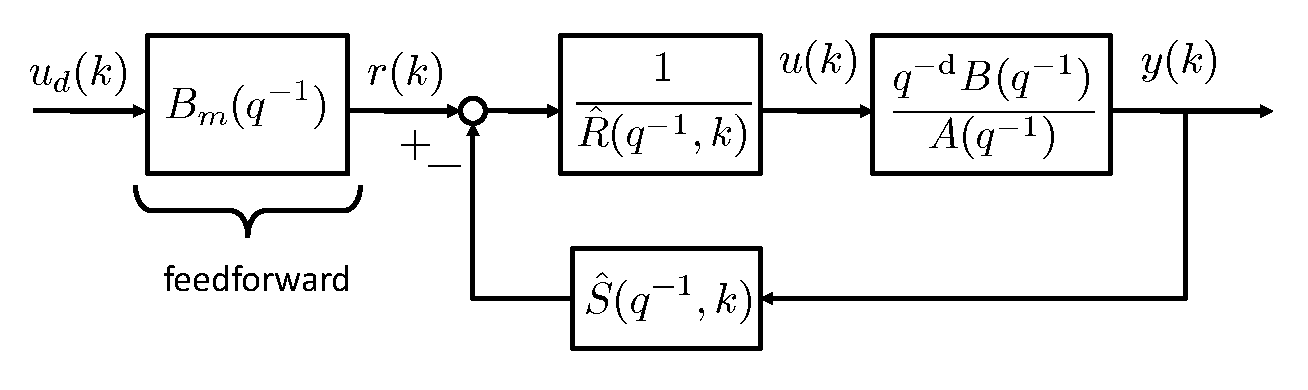
\includegraphics[width=8cm]{figs_control}\\
        \end{figure}
        \begin{align*}
            \hat{R}(q^{-1},k) u(k) = B_m(q^{-1}) u_d(k) - \hat{S}(q^{-1},k) y(k)
        \end{align*}
        where
        \begin{align*}
            \hat{R}(q^{-1},k) & = \hat{r}_0(k) + \hat{r}_1(k) q^{-1} + \cdots + \hat{r}_{n_r}(k) q^{-n_r} \\
            \hat{S}(q^{-1},k) & = \hat{s}_0(k) + \hat{s}_1(k) q^{-1} + \cdots + \hat{s}_{n_s}(k) q^{-n_s}
        \end{align*}

    \end{enumerate}
\end{frame}




